\documentclass{beamer}

\setlength{\leftmargini}{1em}
\setbeamertemplate{itemize item}[circle]
\setbeamertemplate{frametitle}
{
\raggedright\insertframetitle%
}

\usepackage{lipsum}

\usepackage{agda}
\usepackage{apacite}
\usepackage{catchfilebetweentags}
\usepackage{changepage}
\usepackage{babel}
\usepackage{bookmark}

\usepackage{graphicx}

\usepackage[autostyle=true,french=guillemets,maxlevel=3]{csquotes}

\graphicspath{ {images/} }

\usepackage{newunicodechar}
\newunicodechar{∋}{$\ni$}
% \newunicodechar{·}{$\cdot$}
\newunicodechar{⊢}{$\vdash$}
\newunicodechar{⋆}{${}^\star$}
\newunicodechar{Π}{$\Pi$}
\newunicodechar{⇒}{$\Rightarrow$}
\newunicodechar{ƛ}{$\lambdabar$}
\newunicodechar{∅}{$\emptyset$}
\newunicodechar{∀}{$\forall$}
\newunicodechar{ϕ}{$\Phi$}
\newunicodechar{ψ}{$\Psi$}
\newunicodechar{ρ}{$\rho$}
\newunicodechar{α}{$\alpha$}
\newunicodechar{β}{$\beta$}
\newunicodechar{μ}{$\mu$}
\newunicodechar{σ}{$\sigma$}
\newunicodechar{≡}{$\equiv$}
\newunicodechar{Γ}{$\Gamma$}
\newunicodechar{∥}{$\parallel$}
\newunicodechar{Λ}{$\Lambda$}
\newunicodechar{₀}{$~_0$}
\newunicodechar{₁}{$~_1$}
\newunicodechar{₂}{$~_2$}
\newunicodechar{₃}{$~_3$}
\newunicodechar{θ}{$\theta$}
\newunicodechar{Θ}{$\Theta$}
\newunicodechar{∘}{$\circ$}
\newunicodechar{Δ}{$\Delta$}
\newunicodechar{λ}{$\lambda$}
\newunicodechar{⊧}{$\models$}
\newunicodechar{⊎}{$\uplus$}
\newunicodechar{η}{$\eta$}
\newunicodechar{⊥}{$\bot$}
\newunicodechar{Σ}{$\Sigma$}
\newunicodechar{ξ}{$\xi$}
\newunicodechar{ℕ}{$\mathbb{N}$}
\newunicodechar{ᶜ}{${}^c$}
\newunicodechar{Φ}{$\Phi$}
\newunicodechar{Ψ}{$\Psi$}
\newunicodechar{⊤}{$\top$}
\newunicodechar{≐}{$\doteq$}
\newunicodechar{≣}{$\triangleq$}
\newunicodechar{≃}{$\simeq$}
\newunicodechar{≅}{$\cong$}
\newunicodechar{∙}{$\bullet$}
\newunicodechar{ℓ}{$\ell$}
\newunicodechar{ℚ}{$\Q$}
\newunicodechar{ℤ}{$\Z$}
\newunicodechar{⦃}{$\{$}
\newunicodechar{⦄}{$\}$}
\newunicodechar{≤}{$\leqslant$}
\newunicodechar{≥}{$\geqslant$}
\newunicodechar{≟}{$\doteq$}
\newunicodechar{∈}{$\in$}
\newunicodechar{↣}{$\rightarrowtail$}
% \newunicodechar{}{$$}


\newunicodechar{∣}{\ensuremath{\mathnormal{\|}}}
\newunicodechar{∷}{\ensuremath{::}}

\newcommand{\agda}[2]{\ExecuteMetaData[latex/#1.tex]{#2}}

\usetheme{Frankfurt}

\DeclareQuoteStyle{english}
  {\em}
    {\em}
    {\textquotedblleft\em}
    {\em\textquotedblright}

% Information to be included in the title page:
\title{Formalizing Bitcoin prototype \\
  using dependent types in Agda }
\author[Guilherme H. A. Silva]{Guilherme Horta Alvares da Silva}
% \institute{Fundação Getulio Vargas}
\date{2021}


\begin{document}

\frame{\titlepage}

\section{Introduction}

\begin{frame}
\frametitle{Goal}
\begin{itemize}
  \item Using Agda's dependent types to create a formal definition of a crypto currency similar to Bitcoin.
    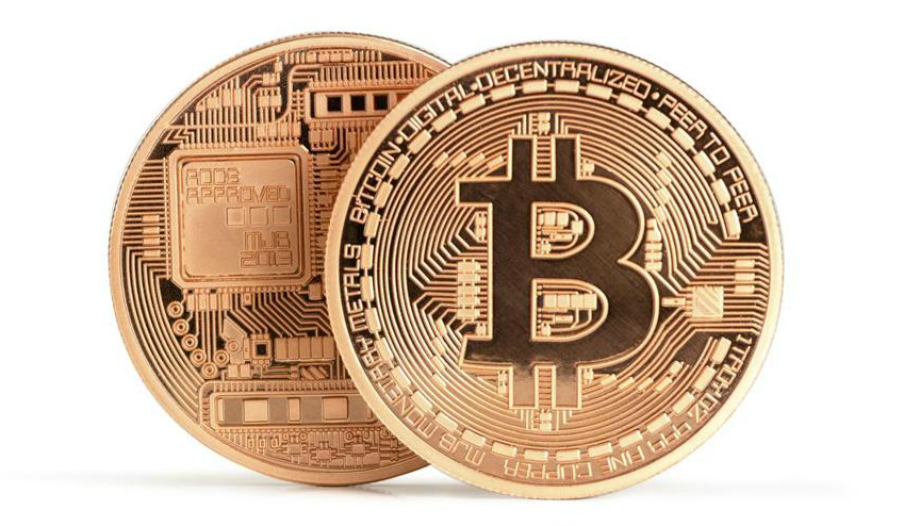
\includegraphics[width=8cm, height=5cm]{TwoBitcoins}
\end{itemize}
\end{frame}

\begin{frame}
   \frametitle{Definition}
\begin{itemize}[<+->]
     \item A cryptocurrency is a decentralized mean of exchange that uses
       blockchain and cryptography to create new currency units and ensure the validity of transactions.
     \item Bitcoin is considered the world's first decentralized digital currency,
       constituting an alternative economic system (peer-to-peer electronic cash system).
       % \cite{nakamoto2008bitcoin}
     \item In this project, I will define cryptographic functions, transactions, block and blockchain.
     \item Distributed system aspects are outside of the scope of this work.
     \end{itemize}
\end{frame}

\begin{frame}
   \frametitle{Ethical Aspects}
\begin{itemize}[<+->]
  \item In Satoshi Nakamoto's vision, Bitcoin would be mined by everyone.
    But until today, there are just a few miners on Earth.
  \item Mining spends a lot of energy because of the proof of work of Bitcoin.
    However, most of the energy to mine is green. It is usually geothermic energy that would not be used where it was produced.
  \item Other cryptocurrencies, such as Cardano, use Proof of Stake to solve this problem. In addition, mining rewards go to people who have a Proof of Stake cryptocurrency.
\end{itemize}
\end{frame}

\begin{frame}
  \frametitle{Imports}
\begin{code}

module main where

open import Level using (Level)
open import Data.Nat
open import Data.List
open import Data.Unit using (⊤; tt)
open import Data.Empty
open import Data.Sum hiding (map)
open import Data.Fin hiding (_+_; _≥_; _≤_; _-_; _≟_)
open import Data.Product hiding (map)
open import Function renaming (Injective to InjectiveSetoid)
open import Relation.Binary.PropositionalEquality
open import Relation.Nullary
open import Utils
\end{code}
\end{frame}

\section{Crypto Functions}

\begin{frame}
  \frametitle{Bitcoin Account}
    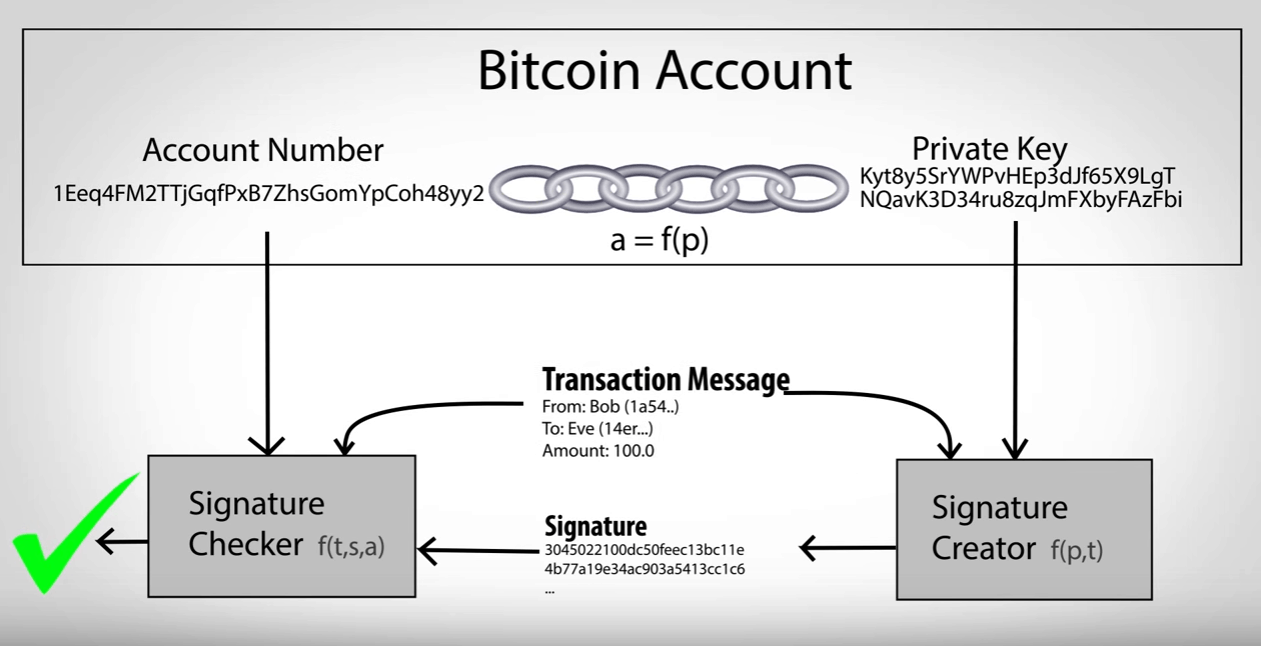
\includegraphics[width=11cm, height=7cm]{privatekey}
\end{frame}

\begin{frame}
  \frametitle{Hash Function}
  \begin{itemize}[<+->]
    \item A hash function serves to fingerprint large data into a number.
    \item It is assumed that two different files will always have different hashes (injectivity)
   since the probability of two different files having the same hash is negligible.
    \item By the pigeonhole principle, the injectivity of the hash is impossible.
      However, two files that have the same hash were never found in SHA-256.
    \item It is also not possible to compute the inverse of the hash function.
  \end{itemize}
\end{frame}

\begin{frame}
  \frametitle{Cryptographic Functions}
  \begin{itemize}[<+->]
    \item In Bitcoin, there is a private and a public key.
    \item From the private key, it is possible to generate a public key
 and to sign a transaction.
    \item It is not possible to know the private key from the public key and signature generated by it.
    \item It is possible to know if a signature and a public key coincide with the same private key that generates both of them.
    \item These functions are based on the SHA-256 hash function.
  \end{itemize}
\end{frame}

\AgdaHide{
\begin{code}
private variable
  ℓ : Level
  A B : Set ℓ
  MSG : Set
\end{code}
}

\begin{frame}
  \frametitle{Hashable}
\begin{code}
Hashable : Set ℓ → Set ℓ
Hashable A = A ↣ ℕ

instance
  open Injection hiding (cong)

  Hashableℕ : Hashable ℕ
  to Hashableℕ = id
  Injection.cong Hashableℕ refl = refl
  injective Hashableℕ refl = refl

Injective : (A → B) → Set _
Injective = InjectiveSetoid _≡_ _≡_

isHashFunctionℕ : (f : ℕ → ℕ) → Set
isHashFunctionℕ f = Injective f

HashFunctionℕ : Set
HashFunctionℕ = Σ[ f ∈ (ℕ → ℕ) ] isHashFunctionℕ f

module Hashableℕ (hashFunctionℕ@(hashℕ , _) : HashFunctionℕ) where
  hash : ⦃ Hashable A ⦄ → A → ℕ
  hash ⦃ hashA ⦄ = Injection.to hashA

  hashBoth : ⦃ Hashable A ⦄ → ⦃ Hashable B ⦄ → A → B → ℕ
  hashBoth ⦃ hashA ⦄ ⦃ hashB ⦄ a b = hash (hash a + hash b)
\end{code}


\end{frame}


\begin{frame}
  \frametitle{Crypto Constants}
\begin{code}
  record CriptoSets : Set₁ where
    field
      PrivateKey         : Set
      PublicKey          : Set
      hashablePublicKey  : Hashable PublicKey
      Signature          : Set

    instance
      _ = hashablePublicKey

    Address = ℕ

    address : PublicKey → Address
    address = hash
\end{code}

\end{frame}

\begin{frame}
  \frametitle{Postulates}
  \begin{itemize}[<+->]
    \item Hash injective is impossible to proof.
      But we postulate it because the probability of hash collision is very low.
    \item In my master thesis, each function of crypto was postulated.
      However, it is better to put these functions as variables.
      Therefore, the code can be more general for every crypto function that has these properties.
  \end{itemize}
\end{frame}

\begin{frame}
  \frametitle{Postulates}
  \begin{code}
  record WithCryptoPostulates (cryptoSets : CriptoSets)
    : Set₁ where
    open CriptoSets cryptoSets public
    field
      priv→pub          : PrivateKey → PublicKey
      Signed            : ⦃ Hashable MSG ⦄ → MSG
                          → PublicKey → Signature → Set
      Signed?           : ∀ ⦃ _ : Hashable MSG ⦄ (msg : MSG) pk sig
                          → Dec $ Signed msg pk sig
  \end{code}
\end{frame}

\begin{frame}
  \frametitle{Postulates}
  \begin{code}
  record CryptoPostulates : Set₁ where
    field
      cryptoSets : CriptoSets
      cryptoAxioms : WithCryptoPostulates cryptoSets
    open WithCryptoPostulates cryptoAxioms public

CryptoPostulatesWithHash : Set₁
CryptoPostulatesWithHash = Σ[ hashℕ ∈ _ ]
  Hashableℕ.CryptoPostulates hashℕ
  \end{code}
\end{frame}

\section{Transactions}

\begin{frame}
  \frametitle{Message Signed}
\begin{code}
module _ (cPostulates@(hashℕ , cPosts)
           : CryptoPostulatesWithHash) where

  open Hashableℕ hashℕ
  open CryptoPostulates cPosts

  module _ ⦃ _ : Hashable MSG ⦄ where

    record SignedWithSigPbk  (msg : MSG)
      (publicKey : PublicKey) : Set where
      field
        signature : Signature
        signed    : Signed msg publicKey signature

\end{code}
\end{frame}

\begin{frame}
   \frametitle{Transactions}
   \begin{itemize}[<+->]
     \item With a transaction, it is possible to send Bitcoins from one account to another.
     \item Transactions are like a paper check. The individual specifies an amount and signs the transaction.
     \item In Bitcoin, there are two kinds of transactions:
       the coinbase transactions and the normal transaction.
       There is just one coinbase transaction per block and it has only outputs,
       while the normal transaction has inputs and outputs.
       The inputs of a transaction should be outputs of other transactions that have never been used as input of one transaction.
    \item Furthermore, each transaction must have a signature generated from the private key proving that the public key user agreed to make that transaction.
   \end{itemize}
\end{frame}

\begin{frame}
\begin{code}
  record Transaction : Set where
    field
      publicKeyInput : PublicKey
      addressOutput  : Address
      amount         : ℕ

\end{code}
\end{frame}

\begin{frame}
\begin{code}

  module _ ⦃ _ : Hashable Transaction ⦄ where

    record SignedTransaction  : Set where
      field
        transaction : Transaction
      open Transaction transaction public

      field
        signed : SignedWithSigPbk transaction publicKeyInput

\end{code}
\end{frame}

\section{Blockchain}

\begin{frame}
  \frametitle{Blockchain constants}
\begin{code}
    -- module WithConstants
    --   (totalQtSub1 : ℕ)
    --   (blockReward : BlockPosition → Amount)
    --   where

    --   totalQt : ℕ
    --   totalQt = suc totalQtSub1

    --   tQtTxs : Set
    --   tQtTxs = Fin totalQt
\end{code}
\end{frame}

\AgdaHide{
\begin{code}
record UTXO : Set where
  field
    numberTransaction : ℕ


\end{code}
}


\begin{frame}
   \frametitle{Unspent Transaction Model}
   \begin{itemize}[<+->]
     \item In the unspent transaction model, every transaction is added to the transaction tree.
     \item To find out the balance of an account it is necessary to look at all unspent transactions
       sent to that account.
     \item To transact the currency, it is necessary to use as input the outputs of
       other unspent transactions.
   \end{itemize}
\end{frame}

\begin{frame}
  \frametitle{Bitcoin UTXO}
    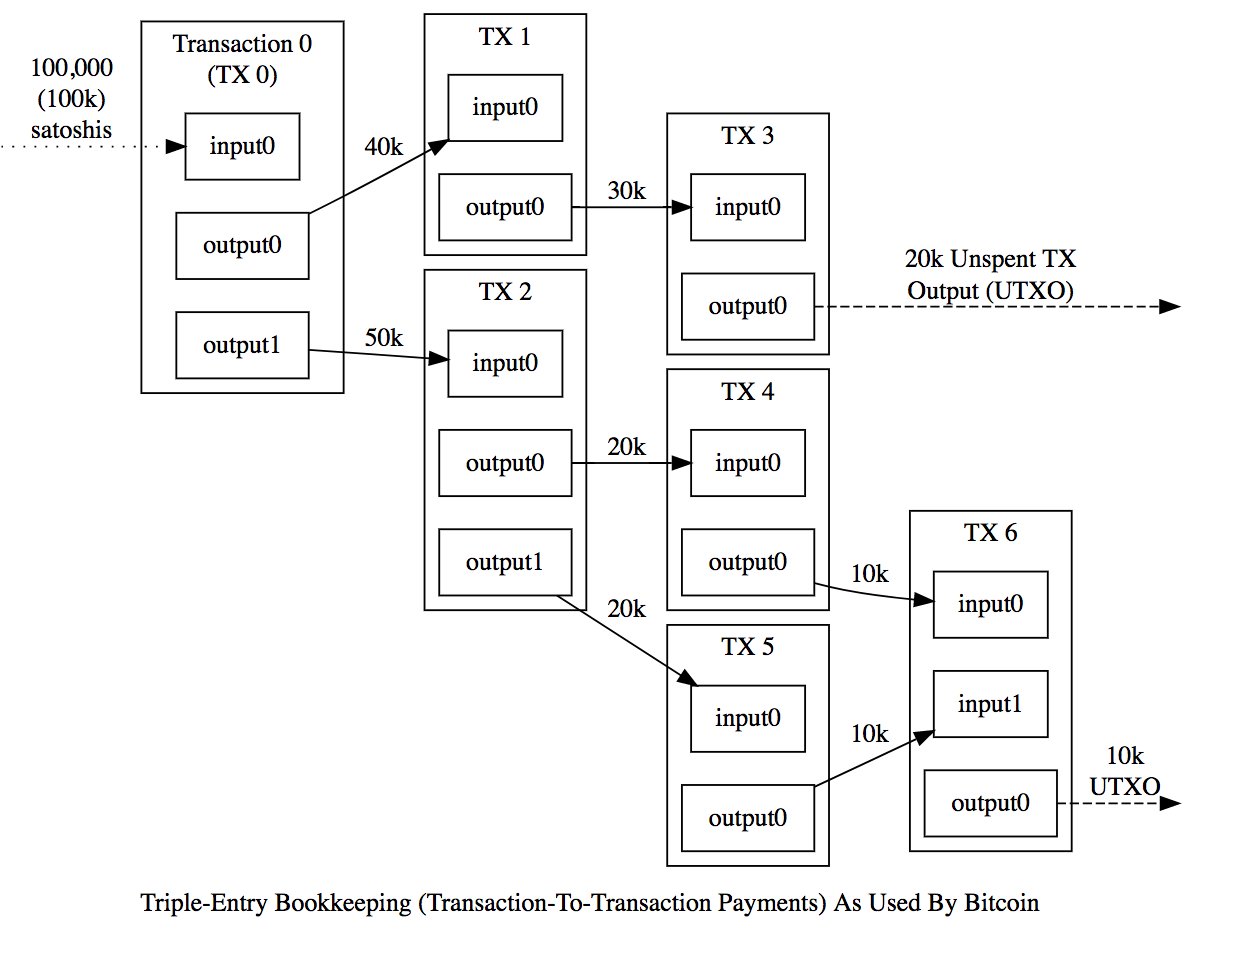
\includegraphics[width=11cm, height=7cm]{utxo}
\end{frame}

\begin{frame}
   \frametitle{Transaction Trees}
   \begin{itemize}[<+->]
     \item The idea of the transaction tree is to gather all transactions into a tree.
     \item In this way, it is possible to fingerprint the information of all transactions calculating just their hash.
     \item With the injectivity property of the hash, it is possible to verify that two trees are equal in constant time complexity.
   \end{itemize}
\end{frame}

\begin{frame}
  \frametitle{Transaction tree}
    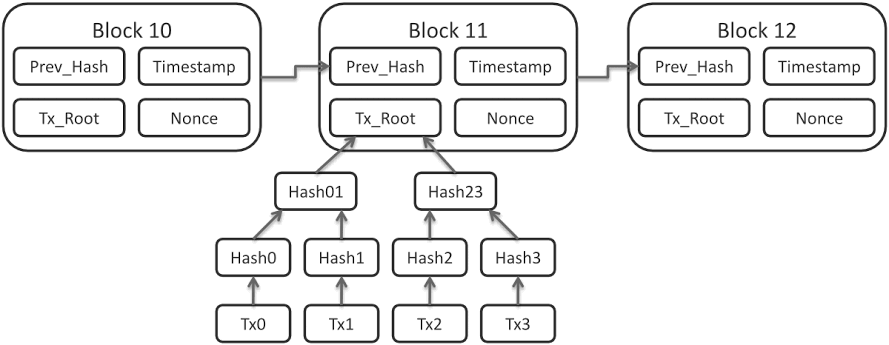
\includegraphics[width=10cm, height=5cm]{blockchain}
\end{frame}


\begin{frame}
   \frametitle{Blocks and Blockchain}
   \begin{itemize}[<+->]
     \item Transactions are embedded in blocks where they are stored.
     \item In Bitcoin, there is a chain of blocks: the blockchain.
       The first block is called the genesis block and every 10 minutes, on average, a new block is added to this blockchain.
     \item There is a limit of transactions that each block can have (in Bitcoin, it is 10 MB of data).
       Therefore, it is important to pay a transaction fee for it to be included in the blockchain.
     \item If there are two blockchains on different computers, it is considered the valid blockchain the one with the most blocks.
   \end{itemize}
\end{frame}

\begin{frame}
\frametitle{Blockchain}
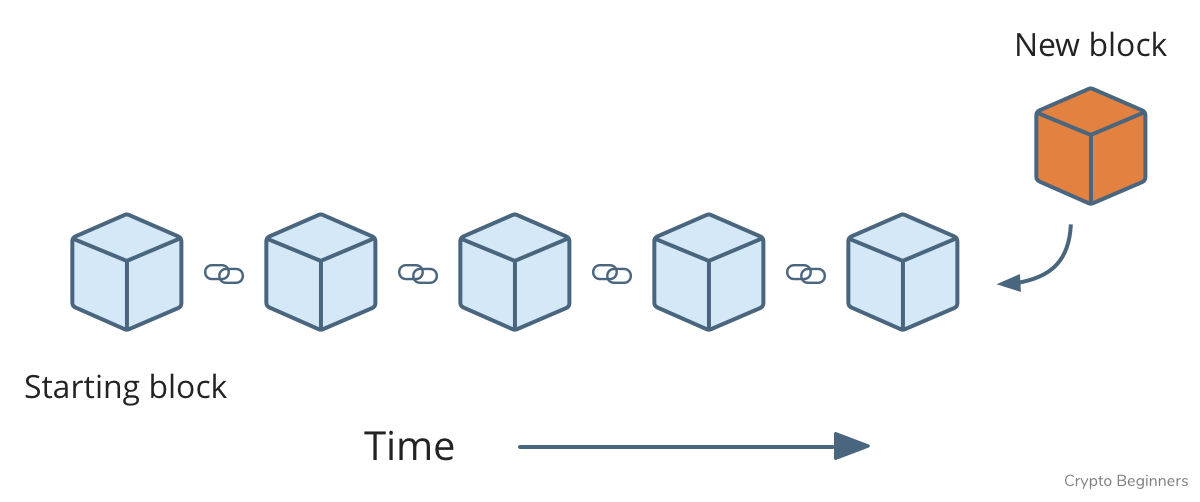
\includegraphics[width=11cm, height=8cm]{blockchain1}
\end{frame}

\begin{frame}
\frametitle{Blockchain}
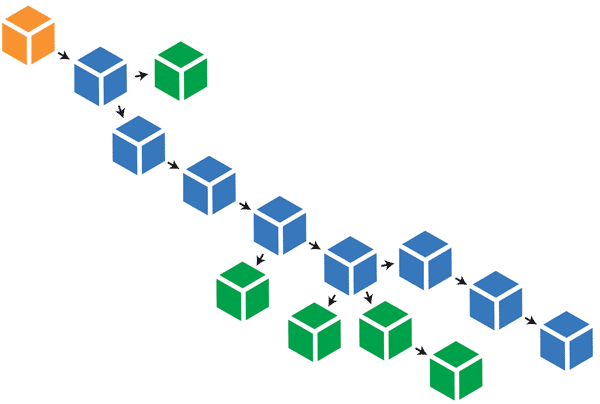
\includegraphics[width=11cm, height=8cm]{blockchain2}
\end{frame}


\begin{frame}
   \frametitle{Mining}
   \begin{itemize}[<+->]
     \item Every block has a cryptographic problem to be solved. That is,
       you need to calculate a nonce value such that the block hash is less than a specified value.
     \item This specified value is calculated from the average of the last 2016 blocks (2 weeks)
       so that the average block mining is 10 minutes.
   \end{itemize}
\end{frame}

\section{Conclusion}

\begin{frame}{Conclusions}
  \begin{itemize}[<+->]
    \item In this work, all specifications were placed on types.
    \item In other works, the approach may be different.
      That is, without any information on types and all proofs done separately.
    \item This approach was not chosen as it is much simpler to understand the code when types are more expressive.
  \end{itemize}
\end{frame}

\begin{frame}{Missing Details}
  \begin{itemize}[<+->]
    \item Calculate block hash and block nounce field.
    \item Change protocol to receive entire block instead of individual transactions.
    \item Substitute the blockchain if there is one larger than it.
  \end{itemize}
\end{frame}

\begin{frame}{More complex parts to add}
  \begin{itemize}[<+->]
    \item Formal modeling of the blockchain as a distributed system.
    \item Create client code to interact with nodes.
    \item Specify the protocol between client and node and between node to node.
          However, adding the evidence to the raw data that the client sends has already been coded,
          which is the most complex part.
    \item Add a scripting language to the cryptocurrency.
  \end{itemize}
\end{frame}

\section{End}

\begin{frame}
  \vspace*{36 pt}
  \begin{center}
  {\Huge Questions?}
  \end{center}
\end{frame}

% \begin{frame}{Bibliographic references}
%   \bibliographystyle{apacite}
%   \bibliography{References}
% \end{frame}

\end{document}
